\documentclass[a4paper, 12pt]{article}

\usepackage{geometry}
\geometry{a4paper,
total={170mm,257mm},left=2cm,right=2cm,
top=1cm,bottom=2cm}
\usepackage{wrapfig}
\usepackage{graphicx}
\usepackage{mathtext}
\usepackage{amsmath}
\usepackage{siunitx} % Required for alignment
\usepackage{multirow}
\usepackage{gensymb}
\usepackage{rotating}
\sisetup{
  round-mode          = places, % Rounds numbers
  round-precision     = 2, % to 2 places
}

\usepackage[T1,T2A]{fontenc}

\usepackage[russian]{babel}

\graphicspath{{pictures/}}

\author{Каграманян Артемий, Б01-208}
\date{\today}
\title{Лабораторная работа 2.5.1 \\ Измерение коэффициента поверхностного натяжения жидкости }

\begin{document}
\maketitle

\section{Аннотация}
    \textbf{Цель работы:} 1) измерение температурной зависимости  коэффициента поверхностного натяжения дистиллированной воды с использованием известного коэффициента поверхностного натяжения спирта;  2) определение полной поверхностной энергии  и теплоты, необходимой для изотермического образования единицы  поверхности жидкости  при различной температуре.  \\
    
    \textbf{Оборудование:} прибор Ребиндера с термостатом и микроманометром; исследуемые жидкости; стаканы.


\section {Теоретическая справка} 

    Для сферического пузырька с воздухом  внутри жидкости избыточное давление даётся формулой Лапласа:

    \begin{equation}
        \triangle P = P_{внутри} - P_{снаружи} = \dfrac{2\sigma}{R}         
    \end{equation}
    
    \begin{figure}[h]
        \centering
        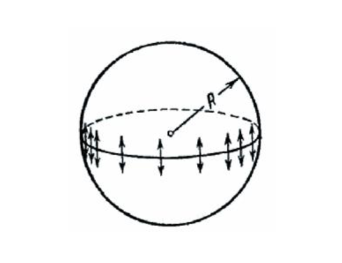
\includegraphics[width=0.2\linewidth]{bubble.png}
    \end{figure}

    где $\sigma$ – коэффициент поверхностного натяжения, $P_{внутри}$ и $Р_{снаружи}$ – давление внутри пузырька и снаружи, R – радиус кривизны поверхности раздела двух фаз.

\section {Методика измерений}

    Исследуемая жидкость (дистиллированная вода) и тестовая жидкость (этиловый спирт) наливаются в сосуд (см. рис. ниже). При создании достаточного  разряжения воздуха в колбе с иглой пузырьки воздуха начинают побулькивать через жидкость. Поверхностное натяжение можно определить по величине разряжения $\triangle P$ (1), необходимого для прохождения пузырьков (при известном радиусе иглы).
    
    Разряжение в системе создается с помощью аспиратора А. Разность давлений в полостях с разряженным воздухом и атмосферой измеряется спиртовым микроманометром.
    Для стабилизации температуры исследуемой жидкости через рубашку D колбы В непрерывно прогоняется вода из термостата.

    \begin{figure}[h]
        \centering
        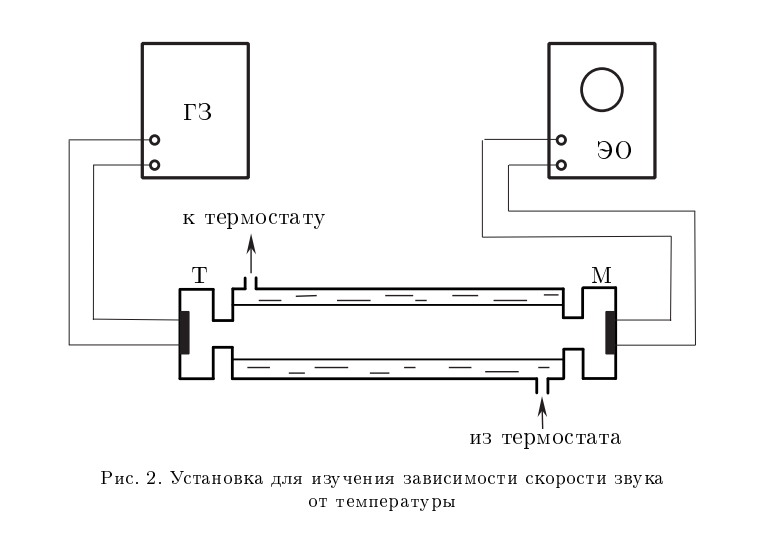
\includegraphics[width=0.7\linewidth]{ust.png}
    \end{figure}
    
\section {Результаты измерений и обработка данных} 

    Убедившись в герметичности системы, начнем измерения. Откроем кран К1 аспиратора и подберем частоту падения капель из него так, чтобы максимальное давление манометра не зависело от этой частоты (не чаще, чем 1 капля в 5 секунд).

    При пробулькивании спирта:
    \[
        \triangle P_{max} = 47 мм.спирт.ст
    \]

    Сделаем несколько пробулькиваний, полученные данные внесем в таблицу и рассчитаем радиус:

    \begin{table}[h]
        \centering
        \begin{tabular}{|c|c|}
            \hline
            $\Delta P$, мм.сп.ст. & $r_{тр}, мм$\\    
            \hline        
            47 & 0.62 \\
            46 & 0.64 \\
            47 & 0.62 \\
            47 & 0.62 \\
            46 & 0.64 \\
            \hline   
        \end{tabular}
    \end{table}

    Тогда получаем радиус:
    \[
        R = 0.63 \pm 0.02 мм
    \]

    Измерив данный радиус микрометром мы получаем значение 0.55 мм. 

    Теперь, утопим иглу на максимальную высоту, оставив небольшое расстояние до дна, чтобы пузырек его не касался.  

    \begin{table}[h]
        \begin{center}
            \begin{tabular}{|c|c|c|c|c|c|}
                \hline
                $h_1$, см & $P_1$, Па & $h_2$, см & $P_2$, Па & $\Delta P$, Па & $\Delta P_{ман}$, Па\\
                \hline
                1.9 & 132 & 0.65 & 175 & 126.5 & 122.6\\
                \hline
            \end{tabular}
        \end{center}
    \end{table}

    Теперь, построим графики трех величин и сравним наши коэффициенты с табличными:

    \begin{figure}[h]
        \centering
        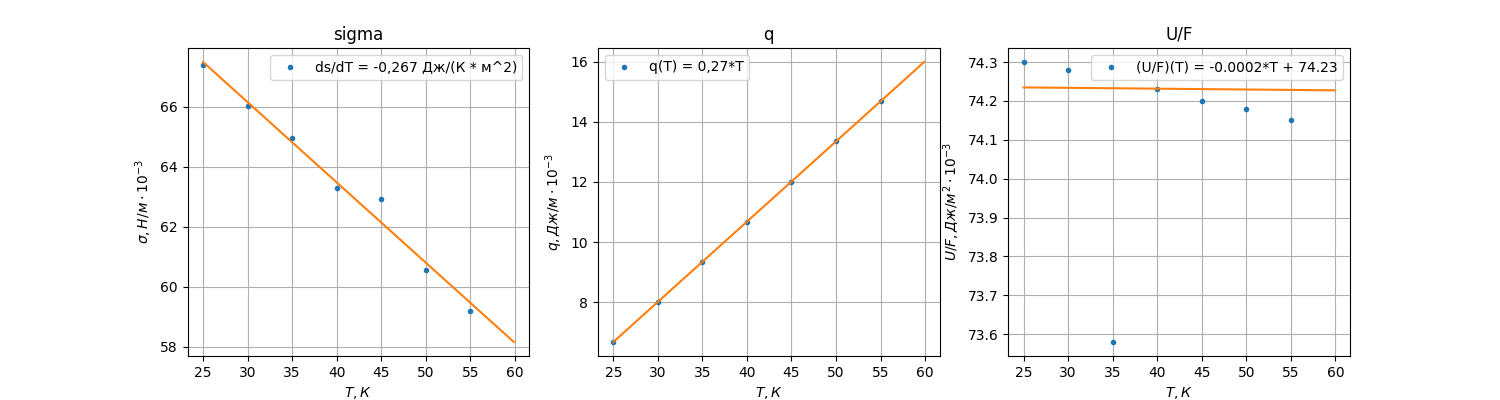
\includegraphics[width = 1.1\linewidth]{sigma.png}
    \end{figure}  

    Видим, все значения отличаются на небольшую константу, это связано с проблемами измерения радиуса иглы.

    По посчитанным данным построим графики, проаппроксимируя их:
  
    
\section {Заключение}
    В данной работе мы научились довольно точно измерять коэффициент поверхностного натяжения жидкости, а именно дистиллированной воды. 
\end{document}